\documentclass[12pt]{article}
\usepackage[utf8]{inputenc}
\usepackage{graphicx}
\usepackage{geometry}
\geometry{a4paper, margin=1in}
\usepackage{times}
\usepackage{titlesec}
\usepackage{cite}
\usepackage{amsmath,amssymb,amsfonts}
\usepackage{algorithmic}
\usepackage{textcomp}
\usepackage{xcolor}
\usepackage{hyperref}
\usepackage{tikz}
\usetikzlibrary{shapes.geometric, arrows}

% TikZ Styles for Flowchart
\tikzstyle{startstop} = [rectangle, rounded corners, minimum width=2cm, minimum height=0.5cm,text centered, draw=black, fill=red!30]
\tikzstyle{process} = [rectangle, minimum width=2cm, minimum height=0.5cm, text centered, draw=black, fill=orange!30]
\tikzstyle{decision} = [diamond, minimum width=2cm, minimum height=0.5cm, text centered, draw=black, fill=green!30]
\tikzstyle{arrow} = [thick,->,>=stealth]

% Formatting sections to be flush left with numbers, similar to screenshot
\titleformat{\section}{\large\bfseries}{\thesection.}{0.5em}{}
\titleformat{\subsection}{\normalsize\bfseries}{\thesubsection}{0.5em}{}

\begin{document}

\noindent{\Large\bfseries Smart Bed Monitoring for Patient Safety: Using Piezoelectric Sensors and ThingsBoard for Real-Time Care\par}
\vspace{1.5em}

\noindent\textit{1\textsuperscript{st} Anshul Parate, 2\textsuperscript{nd} Aashwath Yadav }\\[1em]
\noindent Department of CSE (AI \& ML), Ramdeobaba University, Nagpur, India.\\[1em]
\noindent Email: anshulnparateweb@gmail.com, yadavar\_7@rknec.edu
\vspace{1.5em}

\noindent{\large\bfseries Abstract}\\[0.5em]
\noindent Caring for patients who have a time moving around is a big problem for hospitals. Nurses have a time keeping an eye on every single bed all the time, which can lead to accidents like falls or sores on the skin.In this project we made a system to watch over patients. This system uses sensors and an ESP32 to see how patients are moving without bothering them.We tried out our idea using a Wokwi simulation. Each sensor takes in information about pressure. Turns it into detailed data.This helped us figure out a line to know when a patient is in bed or when they are moving around a lot.We linked our system to the ThingsBoard platform. This made a dashboard that shows the pressure now and what the patient was doing before.Our tests showed that if we check on the patient every 5 seconds we can give nurses an reliable tool to help keep patients safe.We think this tool can really help nurses take care of patients who cannot move easily.The patient movement system we made is a way to watch over patients without being in their face all the time.This is good, for patients who need a lot of care and for nurses who want to do their job.\par
\vspace{1em}

\noindent\textbf{Keywords:} IoT, Smart Bed, Patient Monitoring, Piezoelectric Sensors, ThingsBoard, ESP32, Healthcare Technology.

\section{Introduction}
We all know it's tough for hospital staff to keep an eye on every patient all the time. Patients who are stuck in bed can get hurt easily if they try to move or get up without help. Many systems try to help. They often use cameras or wearable sensors that patients find annoying.In our project we wanted to create something that works quietly in the background. We picked piezoelectric sensors because they are really thin and can detect small changes in pressure. From what we've seen in research these sensors are being used for lots of things like tracking heartbeats and detecting when someone gets out of bed.These piezoelectric sensors are really sensitive, to pressure. They can detect pressure changes. Piezoelectric sensors are being used a lot for various healthcare applications \cite{peng2019detection, kagawa2013bed, allataifeh2020simultaneous, sethi2017internet, martinez2021iot}. Our goal was to take this technology and connect it to a platform like ThingsBoard. This way healthcare providers can look at data that makes sense to them. We want to make it easy for healthcare providers to understand the data, from this technology \cite{hackster2025esp32, thingsboard_healthcare, allam2023recent, iot_healthcare_patterns, thingsboard_docs}.

\section{Building the Prototype}
\subsection{The Hardware Setup}
Our system is built around the ESP32 microcontroller, which is widely used in IoT healthcare frameworks \cite{esp32_tech_ref, makhani2021esp32, kumar2022iot, sharma2020portable}. We used three piezoelectric sensor modules. Placed them at the Left, Center and Right zones of the bed. We wanted to see how intense the pressure really was. So we did not just want a "yes/no" signal. Instead we made the simulation (available at \url{https://wokwi.com/projects/458486908034788353}) give us analog values. This gave us a range from 0 to 4095 on the ESP32s 12-bit ADC. Now we could see small changes in weight. The ESP32 microcontroller helped us do that.

\begin{figure}[h]
    \centering
    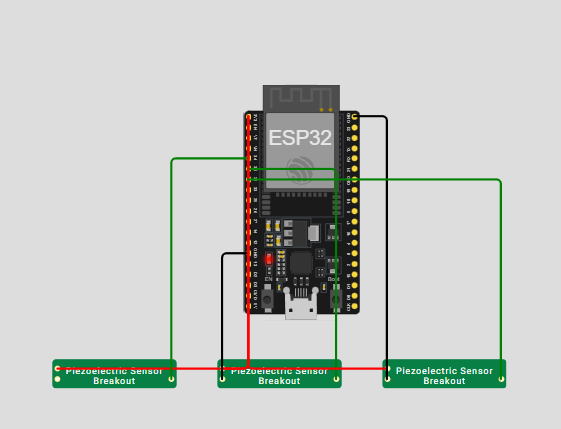
\includegraphics[width=0.45\textwidth]{esp.png}
    \caption{The Wokwi simulation layout where we tested the ESP32 and sensor wiring.}
    \label{fig:circuit}
\end{figure}

\begin{figure}[h]
    \centering
    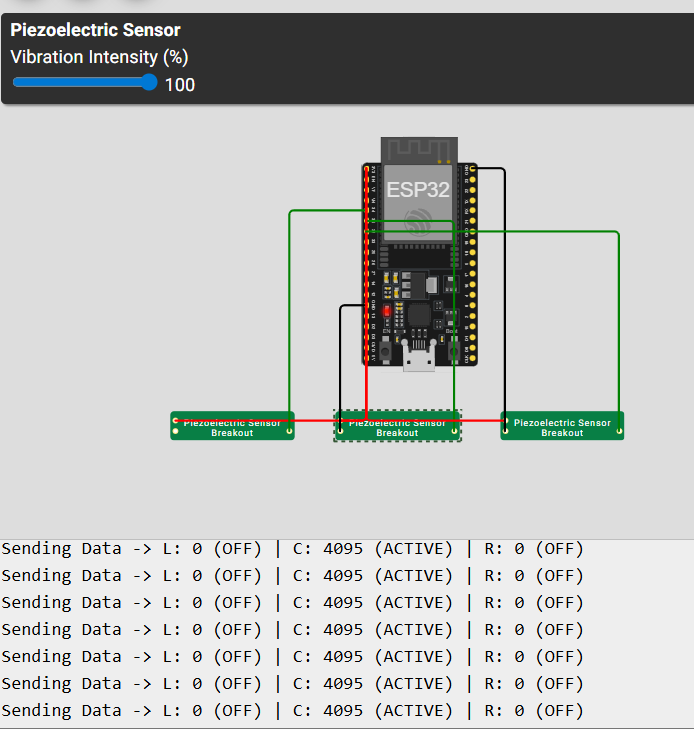
\includegraphics[width=0.45\textwidth]{esp_check.png}
    \caption{Serial Monitor output showing the local processing of sensor data segments.}
    \label{fig:serial}
\end{figure}

\subsection{The Software Logic}
The ESP32 code is quite easy. It does the job. The ESP32 reads the sensors. Checks the values against a certain limit. When we tested the ESP32 we figured out that a value of 500 is just right. This value is low enough to know when someone is lying down. It is high enough to ignore tiny movements or other noise. The ESP32 collects all the data, from the sensors every 5 seconds. Sends the data to the cloud.

\begin{center}
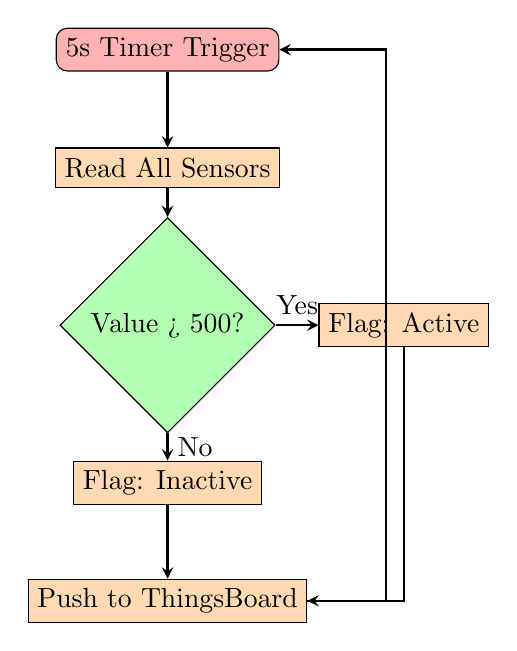
\begin{tikzpicture}[node distance=1.5cm]
    \node (start) [startstop] {5s Timer Trigger};
    \node (read) [process, below of=start] {Read All Sensors};
    \node (check) [decision, below of=read, yshift=-0.5cm] {Value > 500?};
    \node (active) [process, right of=check, xshift=1.5cm] {Flag: Active};
    \node (inactive) [process, below of=check, yshift=-0.5cm] {Flag: Inactive};
    \node (send) [process, below of=inactive] {Push to ThingsBoard};

    \draw [arrow] (start) -- (read);
    \draw [arrow] (read) -- (check);
    \draw [arrow] (check) -- node[anchor=south] {Yes} (active);
    \draw [arrow] (check) -- node[anchor=west] {No} (inactive);
    \draw [arrow] (active) |- (send);
    \draw [arrow] (inactive) -- (send);
    \draw [arrow] (send.east) -- ++(1,0) |- (start.east);
\end{tikzpicture}
\end{center}

\section{Observations and Results}
When we tested the system it was really cool to see how well the sensors caught movement.
The sensors worked great.
They picked up movement well.
It was actually motivating.

\subsection{Live Monitoring}
We created gauges, in the ThingsBoard dashboard. It makes it really easy for a nurse to look at a screen and know if a patient is leaning to one side.. If they are centered.

\begin{figure}[h]
    \centering
    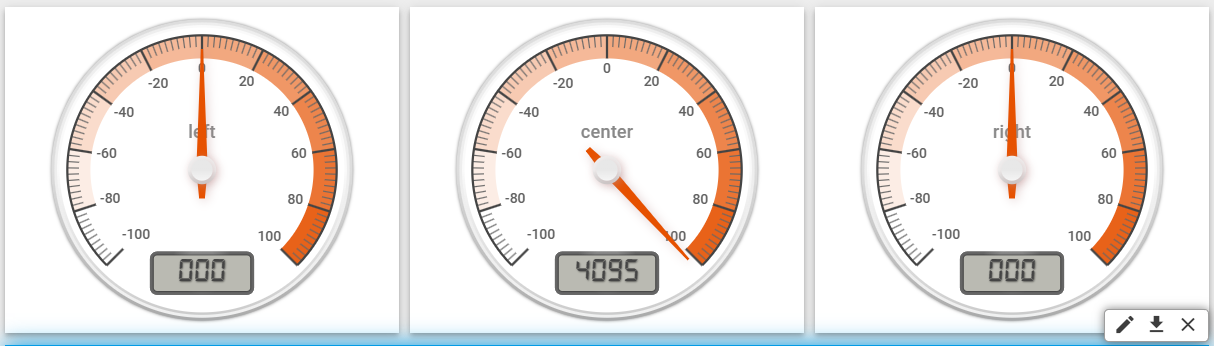
\includegraphics[width=0.48\textwidth]{meter.png}
    \caption{These gauges show the live pressure levels from the three sensors.}
    \label{fig:gauges}
\end{figure}

\begin{figure}[h]
    \centering
    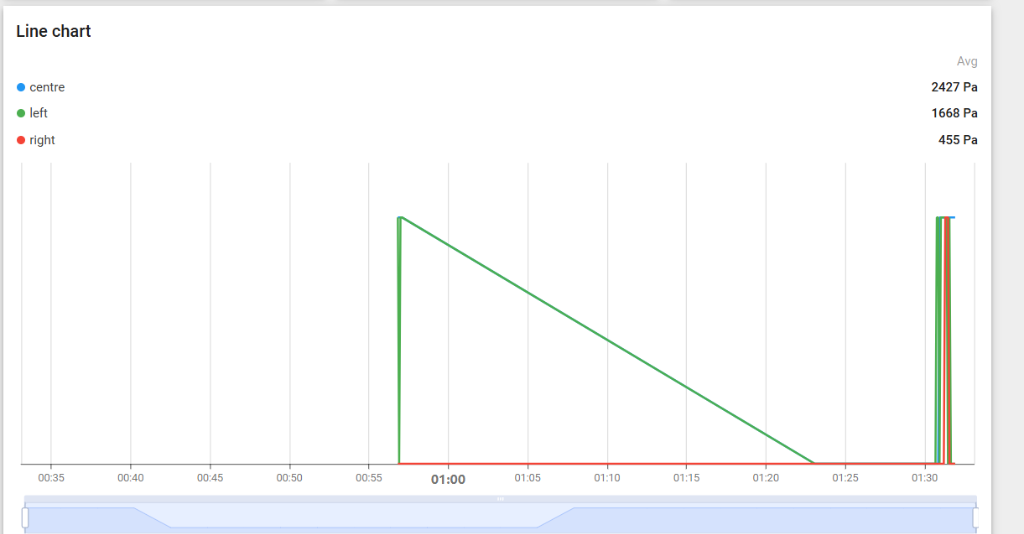
\includegraphics[width=0.48\textwidth]{dashboard_graph.png}
    \caption{Complete dashboard layout uniting real-time gauges with telemetry status.}
    \label{fig:full_dashboard}
\end{figure}

\subsection{Pattern Tracking}
The historical graphs were really helpful in this project.
When I looked at the spikes in the graph I could see when a patient was restless at night. It was easy to track their periods.The graphs, in Fig. \ref{fig:chart},  Showed this information clearly

\begin{figure}[h]
    \centering
    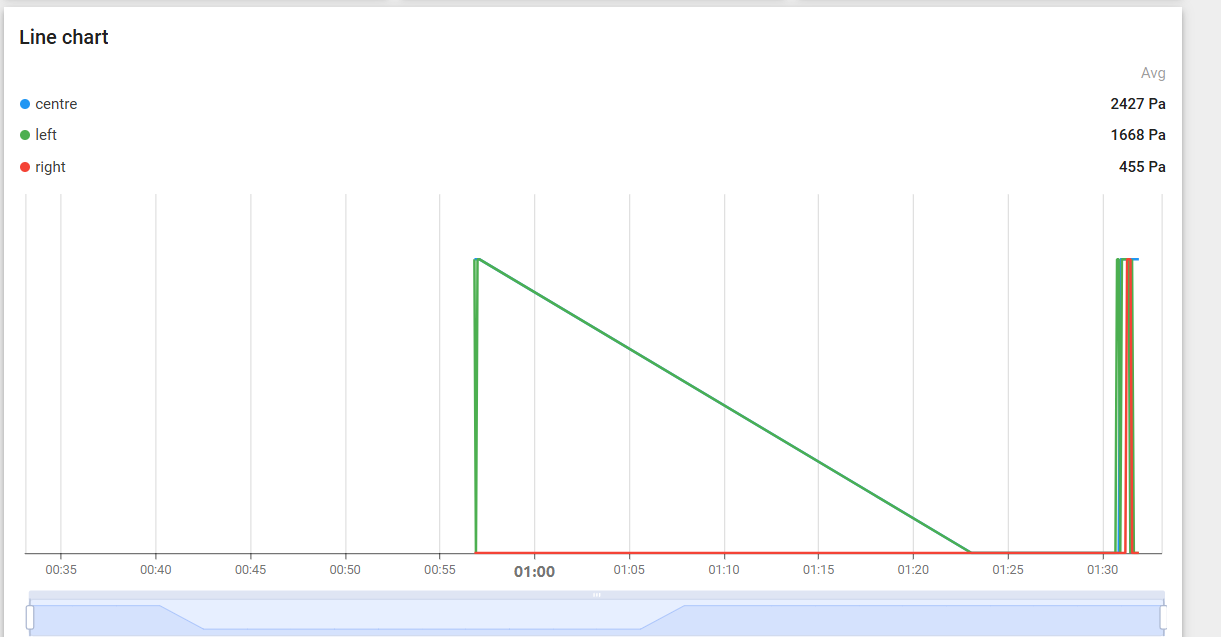
\includegraphics[width=0.48\textwidth]{chart.png}
    \caption{The history chart lets us see exactly when movements happened over time.}
    \label{fig:chart}
\end{figure}

\begin{figure}[h]
    \centering
    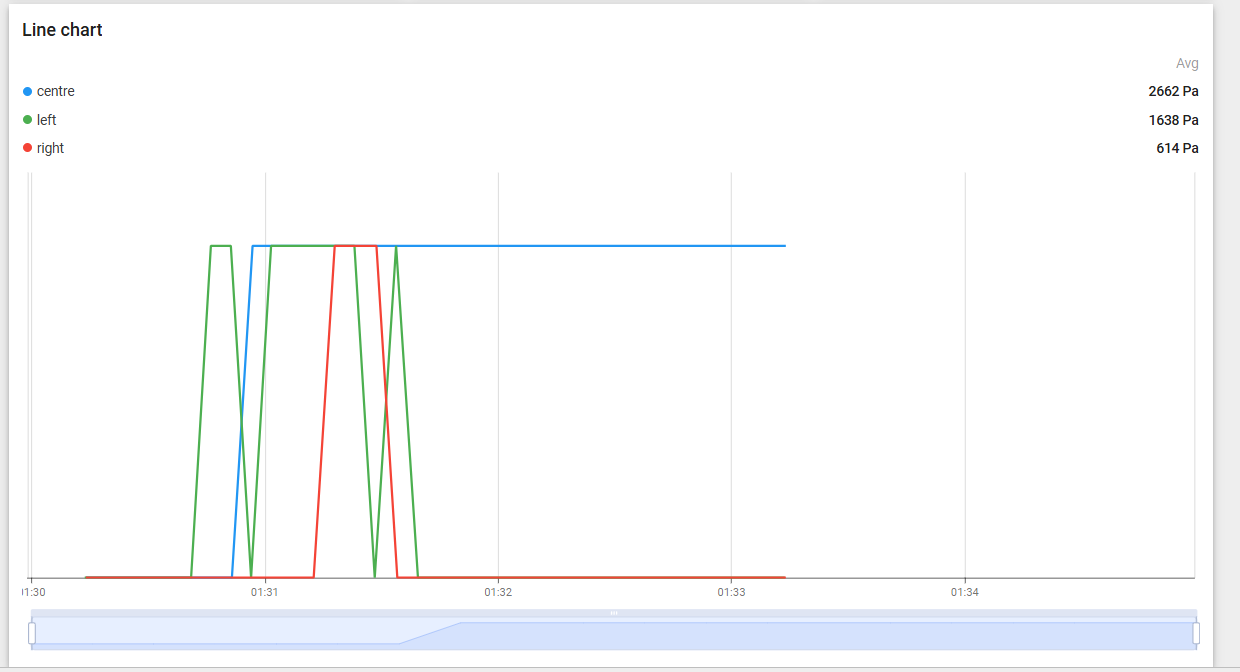
\includegraphics[width=0.48\textwidth]{chart1.png}
    \caption{Close-up view of overlapping sensor signals indicating a patient's shift in position.}
    \label{fig:chart_detail}
\end{figure}

\section{Lessons Learned and Future Goals}
This project showed us that we do not need to buy expensive equipment to make a good monitoring tool. The simple equipment we are using now is good enough to detect what we want. We have some other ideas we want to try. We believe that if we use some machine learning ideas our monitoring tool will be able to detect exactly how a patient is lying in bed or even figure out how fast they are breathing just by feeling the vibrations, in the mattress \cite{donoso2016noninvasive, smart_bed_monitoring_trans, piezo_biosignal_embedded, miguelez2013prediction, sun2022smart, madokoro2018piezoelectric, javaid2021monitoring}. We are talking about the monitoring tool and the same machine learning ideas that we think will help us make it better. The mattress will be a part of this because it is where the patient will be lying and where we will be measuring the vibrations.

\bibliographystyle{plain}
\bibliography{references}

\end{document}
